\documentclass[sigconf]{acmart}
\AtBeginDocument{%
  \providecommand\BibTeX{{%
    \normalfont B\kern-0.5em{\scshape i\kern-0.25em b}\kern-0.8em\TeX}}}

\settopmatter{printacmref=false, printccs=false, printfolios=true}
\setcopyright{none}
\renewcommand\footnotetextcopyrightpermission[1]{}

\makeatletter
\@ACM@nonacmtrue
\renewcommand\@formatdoi[1]{\ignorespaces}
\makeatother

\graphicspath{{./images/}} 
\usepackage{booktabs}
\usepackage{multirow}
\usepackage{tikz}
\usepackage{seqsplit}
\usetikzlibrary{shapes.geometric, arrows, positioning}

\begin{document}

\title{Malware Behavior Comparison: \\
Remote Access Trojan, Fileless, and Living-off-the-Land}
\author{Soleil Cordray}
\email{hi@solcor.dev}
\affiliation{%
  \institution{University of Central Florida}
  \city{Orlando}
  \state{Florida}
  \country{USA}
}

% =============================================================
% ABSTRACT
% =============================================================

\begin{abstract} 

\vspace{0.5em} \qquad This paper presents a comparative static analysis of three malware categories: Remcos Remote Access Trojan (RAT), fileless malware, and living-off-the-land (LotL) attacks. Remcos RAT analysis utilized the Ghidra reverse engineering framework, while fileless and LotL categories were analyzed directly for comparison. The goal was to develop a classification methodology that identifies the behavioral patterns that distinguish each category while noting shared techniques.

\qquad Analysis of a real Remcos RAT sample revealed registry-based persistence through \texttt{RegSetValueExA}, dynamic API loading to evade import analysis, and an embedded C2 URL \\ (\texttt{dsoft1961.narod.ru}). Educational pseudocode samples for fileless and LotL categories were developed based on MITRE ATT\&CK and LOLBAS Project techniques to enable comparison without handling live malware. The results include a behavioral classification table, an Indicators of Compromise (IOC) catalog, and annotated Ghidra screenshots. The analysis shows that while all three categories implement persistence mechanisms, they differ significantly in execution strategy: RATs use compiled binaries with obfuscation, fileless malware operates through scripting engines in memory, and LotL attacks chain trusted Windows utilities.

\vspace{0.5em}
\noindent\textbf{Code \& Artifacts: } \url{https://github.com/soleil-cordray/malware-behavior-comparison}
\end{abstract}

\maketitle
\renewcommand{\shortauthors}{Soleil Cordray}
\renewcommand{\shorttitle}{Malware Behavior Comparison: Remote Access Trojan, Fileless, and Living-off-the-Land}

% =============================================================
% SECTION 1: INTRO & PROB STMT
% =============================================================

\section{Introduction and Problem Statement}

\vspace{0.5em}
\qquad Modern malware has evolved beyond simple executable files that antivirus can easily identify. Three categories give defenders particular difficulty: Remote Access Trojans (RATs) that enable remote system control, fileless malware that runs entirely in memory without dropping files, and living-off-the-land (LotL) attacks that abuse legitimate Windows tools~\cite{lolbas2024project, mitre2024attack}. These threats are difficult to detect because they hide in plain sight using trusted processes, avoid obvious artifacts, and blend into normal system activity~\cite{crowdstrike2024fileless}.

\qquad Remcos RAT is commercially sold as a "remote administration tool" but is widely used for credential theft, keylogging, and maintaining persistent access to compromised systems~\cite{elastic2024remcos}. Security researchers have documented its use by multiple threat actors in phishing campaigns targeting financial institutions, government agencies, and healthcare organizations. The malware supports extensive functionality including screen capture, webcam access, microphone recording, and file system manipulation. Fileless malware takes a different approach, using PowerShell or other scripting engines to run malicious code directly in memory without writing executable files to disk~\cite{crowdstrike2024fileless}. This architectural choice makes traditional file-based scanning inherently ineffective, since there are no malicious files to detect. LotL attacks make detection even harder by using Microsoft-signed tools like \texttt{certutil}, \texttt{mshta}, and \texttt{bitsadmin} to download, execute, and exfiltrate data~\cite{lolbas2024project}. Blocking these tools is impractical because they serve legitimate administrative purposes; security teams must instead monitor suspicious usage patterns.

\qquad This project classifies these malware types through static analysis using Ghidra~\cite{nsacyber2024ghidra} and direct code observation. The goal is to develop a methodology that identifies what makes each category distinct while noting shared techniques. By analyzing a real Remcos sample alongside educational pseudocode samples, the project extracts IOCs and builds a comparison framework applicable to other malware families. The deliverables include annotated Ghidra analysis with screenshots, a behavioral classification table mapping techniques to MITRE ATT\&CK identifiers, and a comprehensive catalog of indicators useful for detection and response.

% =============================================================
% SECTION 2: RELATED WORK
% =============================================================

\section{Related Work}

\vspace{0.5em}
\qquad The LOLBAS Project maintains a comprehensive database documenting abuse patterns for more than 150 legitimate Windows binaries, including \texttt{certutil}, \texttt{mshta}, \texttt{rundll32}, \texttt{bitsadmin}, and \texttt{regsvr32}~\cite{lolbas2024project}. Each entry documents the binary's legitimate purpose, abuse methods, and detection opportunities. MITRE ATT\&CK provides systematic documentation of adversary techniques including signed binary proxy execution (T1218), PowerShell abuse (T1059.001), ingress tool transfer (T1105), and boot/logon auto-start execution (T1547.001)~\cite{mitre2024attack}. These resources informed the development of the sample and its behavioral classification.

\qquad Industry threat intelligence provides operational context. Elastic Security Labs identified Remcos RAT's Delphi-based architecture, encrypted configuration storage, and dynamic API resolution to evade import table analysis~\cite{elastic2024remcos}. Their multi-part analysis series documented specific function addresses responsible for C2 communication, keylogging, and credential theft. CrowdStrike documents PowerShell's role in fileless attacks, including Base64-encoded execution and \texttt{Invoke-Expression} for in-memory payload delivery~\cite{crowdstrike2024fileless}. The Center for Internet Security documents real-world LotL campaigns demonstrating how attackers chain trusted binaries for complete attack life-cycles without deploying custom malware~\cite{cis2024lotl}. Existing ANY.RUN sandbox reports provide dynamic analysis baselines showing Remcos runtime behaviors that include registry modifications, process injection, and network callbacks~\cite{anyrun2024remcos}.

\qquad Ghidra methodologies are well-documented in security research. Varonis provides workflows that emphasize import analysis, string extraction, and cross-reference tracing as the foundational steps towards understanding unknown binaries~\cite{varonis2023ghidra}. Hack The Box outlines the fundamentals of static analysis, including suspicious API identification and behavior reconstruction from disassembly~\cite{htb2024malware}. A foundational text written by Sikorski and Honig, \textit{Practical Malware Analysis}~\cite{sikorski2012practical}, established safe handling practices that informed the isolated VM approach used in this project. Public proof-of-concept implementations such as the bytecode77 repository~\cite{bytecode2024lotl} demonstrate practical fileless attack chains combining PowerShell execution with registry persistence, directly informing the development of this comparison's educational sample. The NSA's release of Ghidra as open-source software~\cite{nsacyber2024ghidra} democratized access to professional-grade reverse engineering capabilities previously limited to expensive commercial tools.

% =============================================================
% SECTION 3: METHODOLOGY
% =============================================================

\section{Methodology}

\vspace{0.5em}
\qquad This project follows three phases: environment configuration, sample acquisition, and static analysis. Figure~\ref{fig:pipeline} illustrates the analysis pipeline. All work was conducted within an isolated virtual machine.

% FIGURE 1
\begin{figure}[h]
\centering
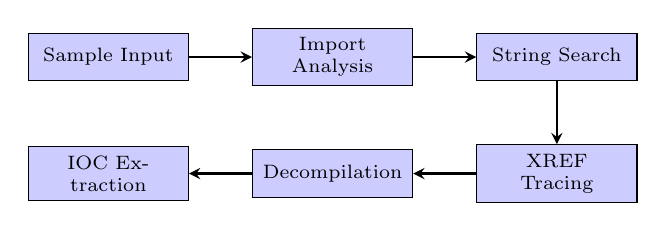
\begin{tikzpicture}[node distance=0.8cm, 
    block/.style={rectangle, draw, fill=blue!20, text width=1.8cm, text centered, minimum height=0.6cm, font=\scriptsize},
    arrow/.style={thick,->,>=stealth}]
\node (input) [block] {Sample Input};
\node (import) [block, right=of input] {Import Analysis};
\node (string) [block, right=of import] {String Search};
\node (xref) [block, below=of string] {XREF Tracing};
\node (decomp) [block, left=of xref] {Decompilation};
\node (output) [block, left=of decomp] {IOC Extraction};
\draw [arrow] (input) -- (import);
\draw [arrow] (import) -- (string);
\draw [arrow] (string) -- (xref);
\draw [arrow] (xref) -- (decomp);
\draw [arrow] (decomp) -- (output);
\end{tikzpicture}
\caption{Static analysis pipeline for IOC extraction.}
\label{fig:pipeline}
\end{figure}

% =============================================================
% SECTION 3.1: ANALYSIS ENVIRONMENT
% =============================================================

\subsection{Analysis Environment}

\vspace{0.5em}
\qquad A Windows 10 Pro VM was deployed in VMware Fusion on a 2019 Intel MacBook Pro. Network isolation was configured through VMware's "Private to my Mac" setting~\cite{vmware2024fusion}, critical when handling live malware. Windows Defender was disabled to prevent sample quarantine. Multiple VM snapshots enabled rapid restoration between sessions. Ghidra 11.0 with OpenJDK 21~\cite{nsacyber2024ghidra}, Notepad++, 7-Zip, and HxD were installed.

% =============================================================
% SECTION 3.2: SAMPLE ACQ. & DEV.
% =============================================================

\subsection{Sample Acquisition and Development}

\vspace{0.5em}
\qquad Three samples were prepared (Table~\ref{tab:samples}). A real Remcos RAT sample was obtained from MalwareBazaar~\cite{malwarebazaar2024} by searching for the tag "RemcosRAT". The SHA256 hash is recorded in the GitHub repository for reproducibility. To avoid handling live malware, fileless and LotL categories are represented by educational pseudocode developed from documented techniques~\cite{bytecode2024lotl, lolbas2024project}.

% TABLE 1
\begin{table}[h]
\caption{Sample Summary}
\label{tab:samples}
\small
\begin{tabular}{@{}llll@{}}
\toprule
\textbf{Category} & \textbf{Type} & \textbf{Source} & \textbf{Tool} \\
\midrule
Remcos RAT & Real binary & MalwareBazaar & Ghidra \\
Fileless & Pseudocode & Custom & Notepad++ \\
LotL & Pseudocode & Custom & Notepad++ \\
\bottomrule
\end{tabular}
\end{table}

\qquad The \textbf{Fileless Loader} pseudocode documents seven stages: (1) error suppression via \texttt{\$ErrorActionPreference}, (2) anti-sandbox environment checks comparing hostnames against analysis patterns, (3) Base64-encoded C2 communication via \\ \texttt{System.Net.WebClient} with browser user-agent spoofing, (4) payload decoding via \texttt{FromBase64String}, (5) in-memory execution via \texttt{Invoke-Expression}, (6) registry persistence through the Run key, and (7) system information exfiltration. Each stage maps to documented MITRE ATT\&CK identifiers.

\qquad The \textbf{LotL sample} documents abuse of nine Windows utilities from LOLBAS~\cite{lolbas2024project}: PowerShell for Defender disabling (T1562.001), \texttt{certutil} for payload download (T1105), \texttt{mshta} for script execution (T1218.005), \texttt{schtasks} for scheduled task persistence (T1053.005), \texttt{rundll32} for LSASS credential dumping (T1003.001), \texttt{reg} for firewall manipulation (T1562.004), \texttt{bitsadmin} for exfiltration via BITS transfers (T1048), \texttt{wevtutil} for Windows event log clearing (T1070.001), and \texttt{regsvr32} for Squiblydoo script execution (T1218.010).

% =============================================================
% SECTION 3.3: GHIDRA ANALYSIS WORKFLOW
% =============================================================

\subsection{Ghidra Analysis Workflow}

\vspace{0.5em}
\qquad Remcos analysis followed six steps based on established methodology~\cite{varonis2023ghidra, htb2024malware}: (1) project setup with auto-analysis (3-4 minutes for the 460KB sample), (2) entry point examination via Function Graph (Figure~\ref{fig:entry}), (3) import table analysis for capability assessment, (4) string search with filters for "http", "Run", and "Software", (5) cross-reference tracing to understand API usage context, and (6) IOC documentation throughout analysis.

% FIGURE 2
\begin{figure}[h]
\centering
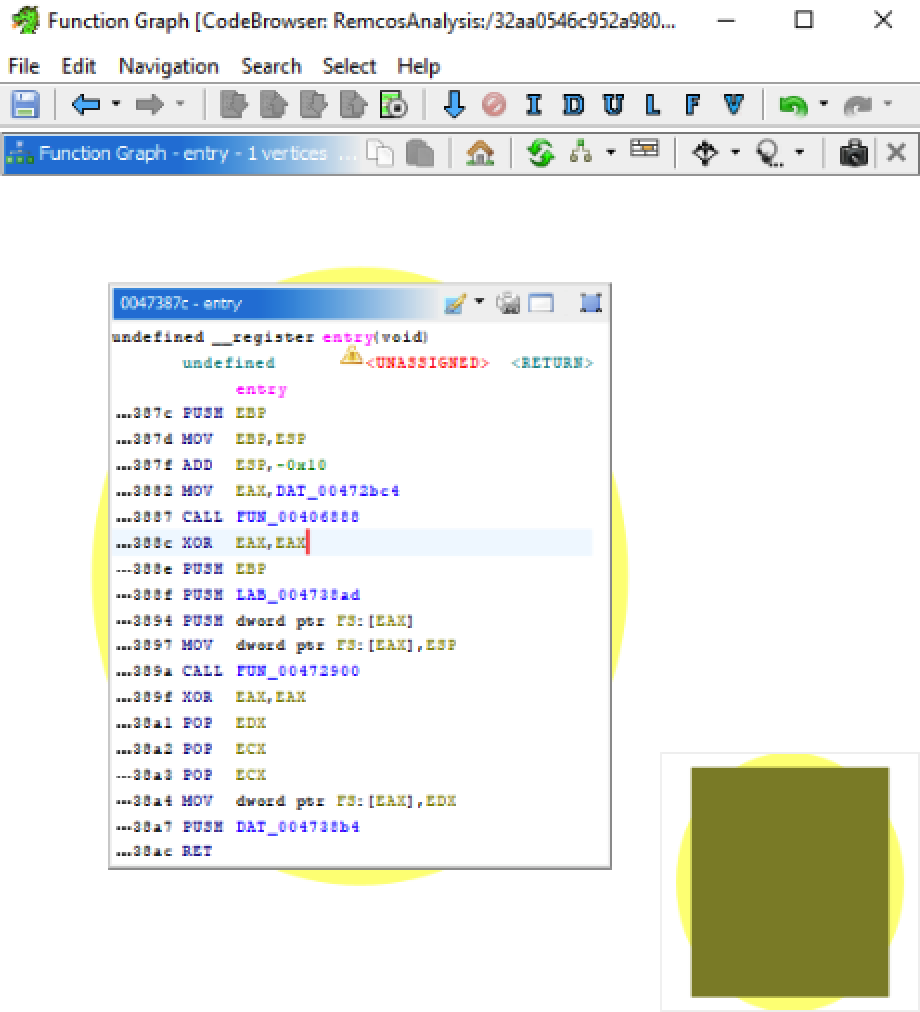
\includegraphics[width=0.42\textwidth]{images/2entry.png}
\caption{Function graph of Remcos entry point showing initial program flow.}
\label{fig:entry}
\end{figure}

% =============================================================
% SECTION 4: EVAL. & RESULTS
% =============================================================

\section{Evaluation and Results}

% =============================================================
% SECTION 4.1: REMCOS RAT BINARY ANALYSIS
% =============================================================

\subsection{Remcos RAT Binary Analysis}

\vspace{0.5em}
\qquad Static analysis of the Remcos sample in Ghidra revealed four significant findings regarding its capabilities and evasion techniques.

\qquad \textbf{Finding 1: Dynamic API Load for Evasion.} The import table (Figure~\ref{fig:imports}) shows ADVAPI32.DLL, COMCTL32.DLL, GDI32.DLL, KERNEL32.DLL, MSIMG32.DLL, OLEAUT32.DLL, \\ SHELL32.DLL, USER32.DLL, VERSION.DLL, and WINMM.DLL. Notably absent are WS2\_32.DLL (Winsock) and WININET.DLL (Internet APIs), which would be expected for a RAT with network capabilities. Since Remcos is documented to have C2 functionality, this absence suggests that the sample resolves networking APIs dynamically at runtime via \texttt{GetProcAddress}---MITRE ATT\&CK technique T1027.007 (Dynamic API Resolution)~\cite{elastic2024remcos}.

% FIGURE 3
\begin{figure}[h]
\centering
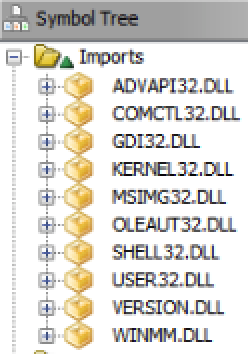
\includegraphics[width=0.33\textwidth]{images/8imports.png}
\caption{Import table lacking networking libraries, indicating dynamic API resolution.}
\label{fig:imports}
\end{figure}

\qquad \textbf{Finding 2: Registry Persistence APIs.} Expanding ADVAPI32.DLL in the imports revealed registry manipulation functions: \texttt{RegCloseKey}, \texttt{RegCreateKeyExA}, \texttt{RegFlushKey}, \\ \texttt{RegOpenKeyExA}, \texttt{RegQueryValueExA}, and \texttt{RegSetValueExA} (Figure~\ref{fig:regapis}). These APIs are commonly used for persistence via the Registry Run key (T1547.001). The complete registry API suite---open, create, query, set, flush, close---indicates sophisticated manipulation capability beyond simple persistence.

\qquad Cross-reference analysis of \texttt{RegSetValueExA} revealed three call locations at the address \texttt{0x00406a18} (Figure~\ref{fig:regxref}). Tracing these XREFs showed that the function was invoked in contexts consistent with persistence establishment. Although the specific registry path was not visible in plaintext (likely encrypted), the API usage pattern strongly suggests Run key persistence~\cite{elastic2024remcos}.

% FIGURE 4
\begin{figure}[h]
\centering
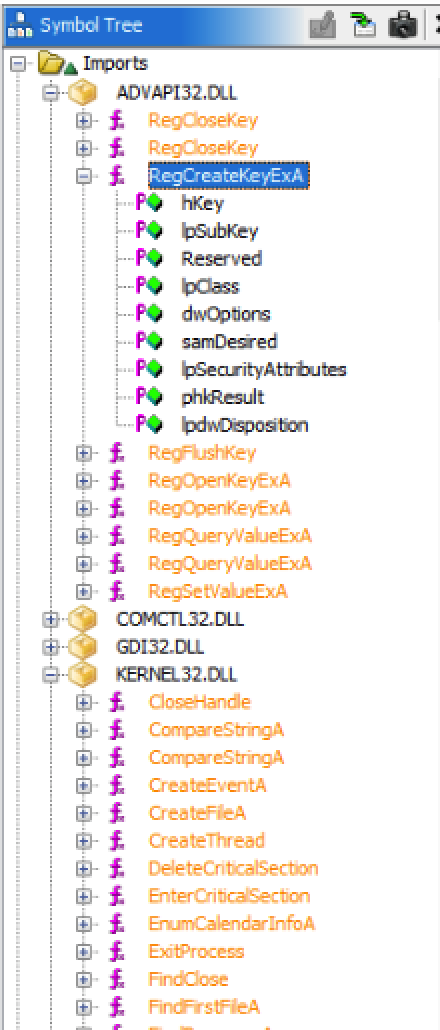
\includegraphics[width=0.33\textwidth]{images/3apis.png}
\caption{ADVAPI32.DLL imports showing registry manipulation APIs.}
\label{fig:regapis}
\end{figure}

% FIGURE 5
\begin{figure}[h]
\centering
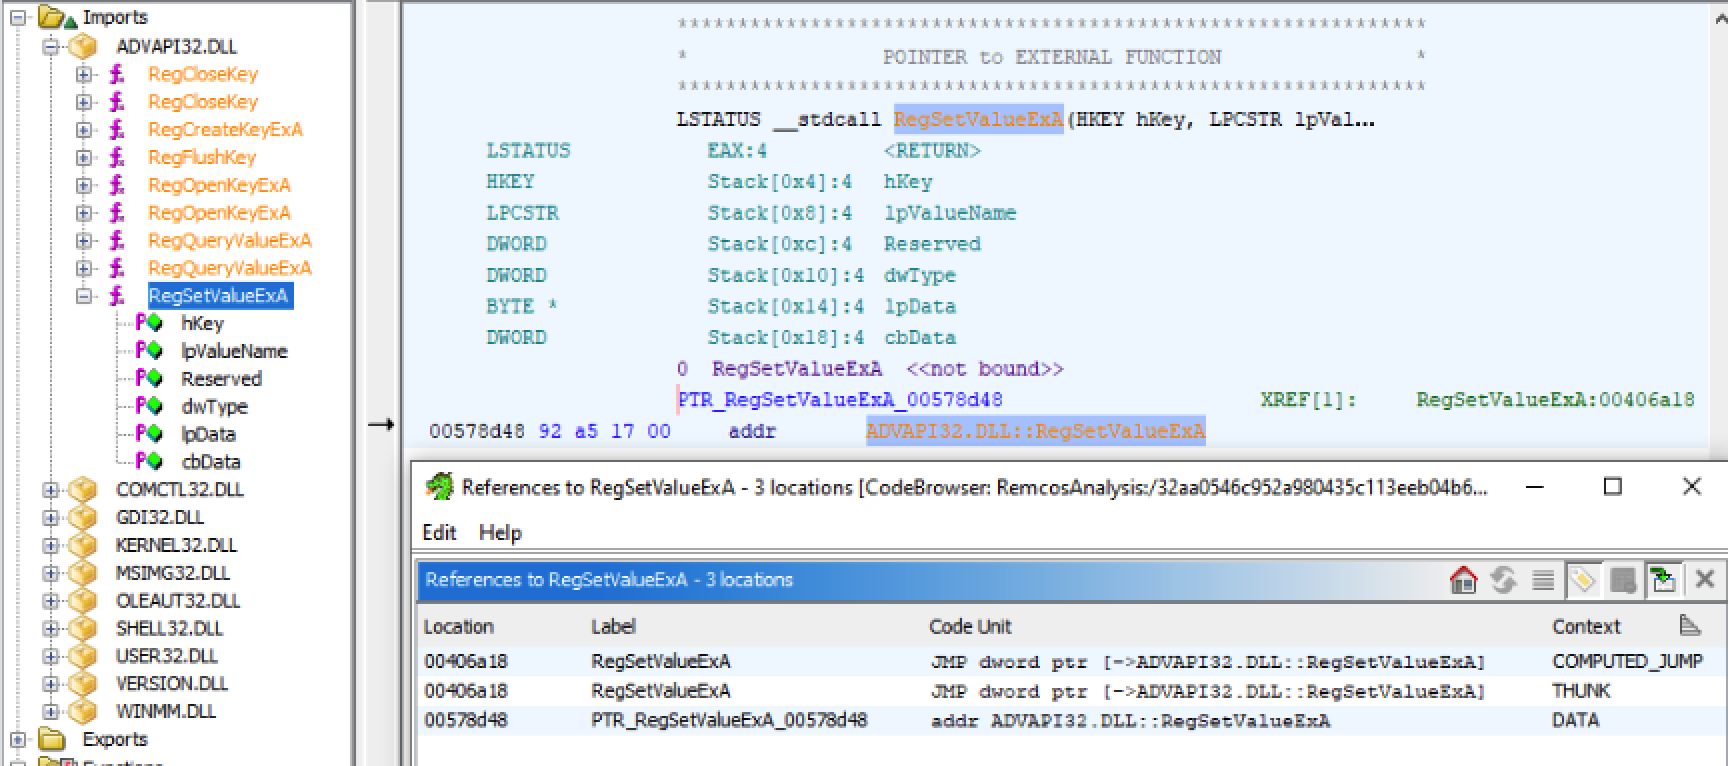
\includegraphics[width=0.46\textwidth]{images/9reg.png}
\caption{Cross-references to RegSetValueExA showing three call locations.}
\label{fig:regxref}
\end{figure}

\qquad \textbf{Finding 3: Embedded C2 URL.} String analysis using Search $\rightarrow$ For Strings with filter "http" revealed an embedded command-and-control URL: \texttt{http://dsoft1961.narod.ru} at the address \texttt{0x004712c0} (Figure~\ref{fig:c2url}). Cross-referencing demonstrated its use by \texttt{FUN\_00470f18}, likely the network initialization routine. The use of a Russian free hosting service is consistent with Remcos infrastructure documentation~\cite{anyrun2024remcos}.

% FIGURE 6
\begin{figure}[h]
\centering
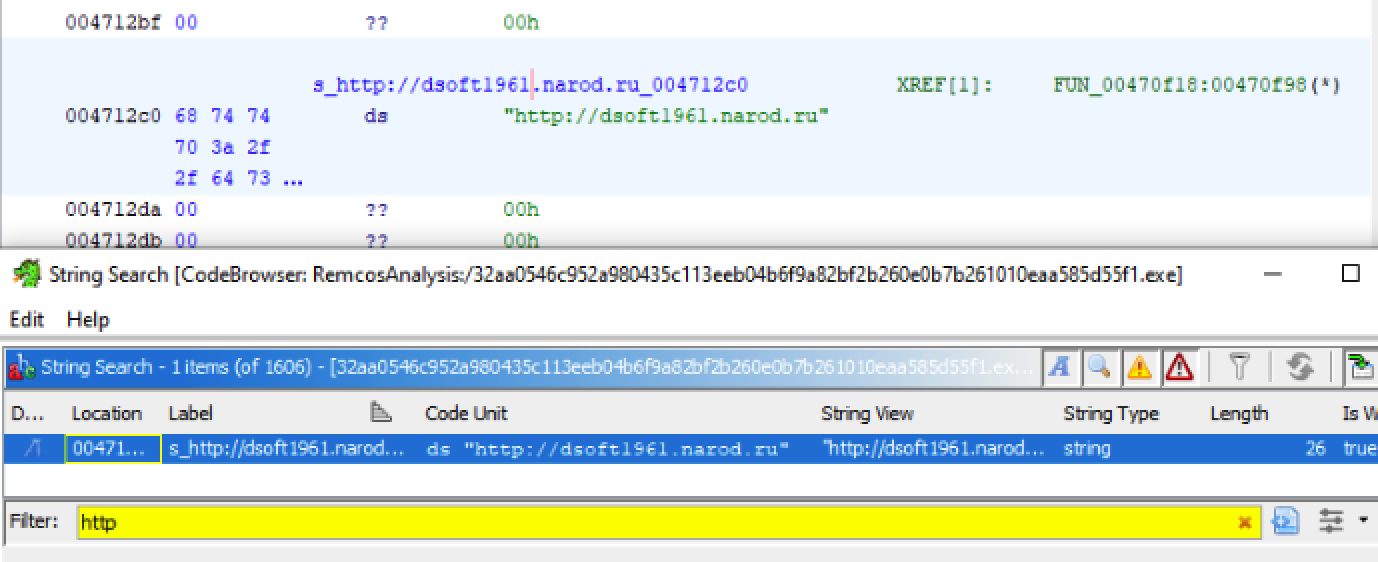
\includegraphics[width=0.46\textwidth]{images/7c2url.png}
\caption{Embedded C2 URL with cross-reference to calling function.}
\label{fig:c2url}
\end{figure}

\qquad \textbf{Finding 4: Delphi Compiler Artifacts.} String analysis revealed Borland Delphi compiler signatures (Figure~\ref{fig:strings}), including "Software\textbackslash Borland\textbackslash Delphi\textbackslash Locales" and "Software\textbackslash DSoft\textbackslash Fifteen". This corroborates Remcos' documented architecture~\cite{elastic2024remcos} and provides additional context for the characteristic import patterns observed in Finding 1.

% FIGURE 7
\begin{figure}[h]
\centering
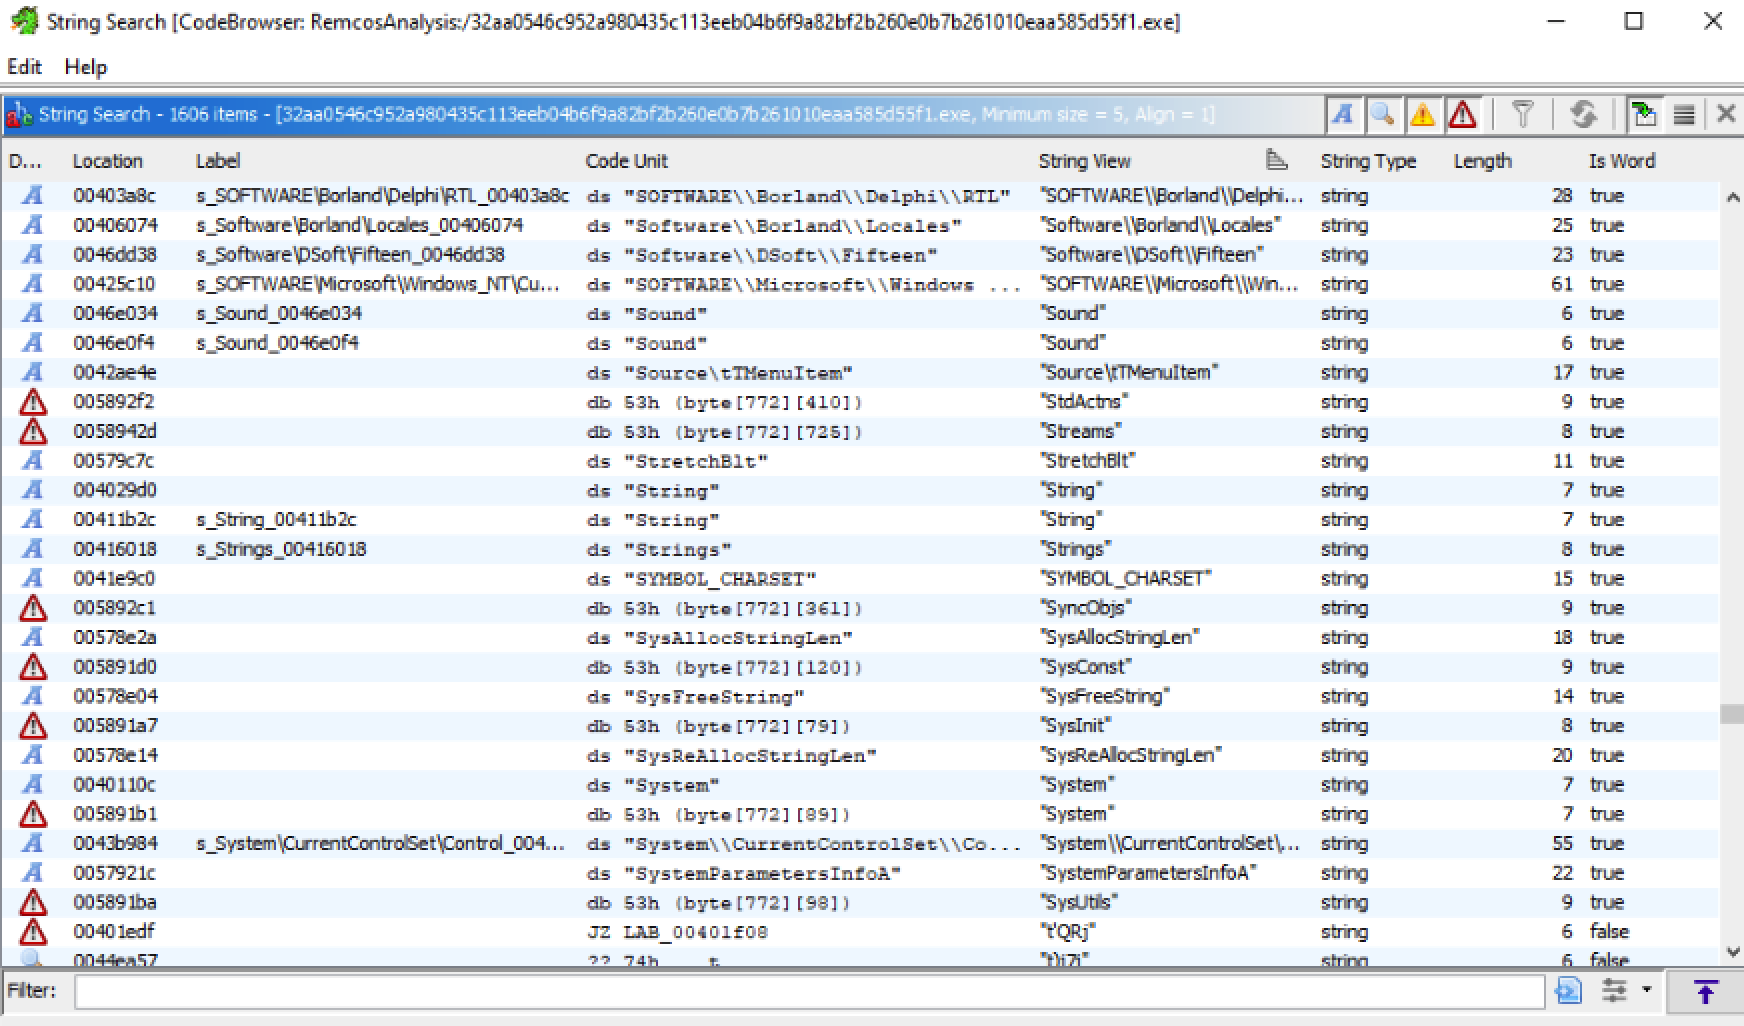
\includegraphics[width=0.46\textwidth]{images/5strings.png}
\caption{Delphi compiler artifacts in string analysis.}
\label{fig:strings}
\end{figure}

% =============================================================
% SECTION 4.2: FILELESS &  LOTL ANALYSIS
% =============================================================

\subsection{Fileless and LotL Analysis}

\vspace{0.5em}
\qquad The fileless pseudocode documents techniques mapped to MITRE ATT\&CK: error suppression (T1562), reconnaissance via environment variables (T1082), C2 configuration with WebClient (T1071), payload download without disk writes (T1105), Base64 decoding (T1140), memory execution via \texttt{Invoke-Expression} (T1059.001), registry persistence (T1547.001), and exfiltration (T1041). The key characteristic distinguishing fileless malware is the complete absence of malicious files on disk; all execution occurs within the PowerShell process memory space, making traditional antivirus file scanning ineffective.

\qquad The LotL pseudocode demonstrates a complete attack chain using Microsoft-signed binaries (Table~\ref{tab:lotl}). Defense evasion occurs first. Disabling Defender ensures that subsequent stages continue uninterrupted. The \texttt{certutil} abuse is particularly effective because it is a legitimate certificate management tool; network security tools often whitelist its traffic patterns. Persistence via \texttt{schtasks} offers significant advantages over registry-based persistence: administrators can specify privilege levels (HIGHEST), configure flexible triggers (ONLOGON, ONSTART, specific times), and scheduled tasks are often harder to enumerate than well-known registry locations. The credential dumping stage via \texttt{rundll32} calling \texttt{comsvcs.dll} MiniDump is a well-documented technique for LSASS memory extraction that can capture plaintext passwords and NTLM hashes. Finally, evidence destruction via \texttt{wevtutil} clearing Security and System logs significantly complicates incident response and forensic investigation.

% TABLE 2
\begin{table}[h]
\caption{LotL Attack Chain---Abused Windows Utilities}
\label{tab:lotl}
\small
\begin{tabular}{@{}p{1.4cm}p{3.3cm}l@{}}
\toprule
\textbf{Binary} & \textbf{Abuse Purpose} & \textbf{ATT\&CK} \\
\midrule
powershell & Disable Defender & T1562.001 \\
certutil & Download payload & T1105 \\
mshta & Execute VBScript & T1218.005 \\
schtasks & Create scheduled task & T1053.005 \\
rundll32 & Dump credentials & T1003.001 \\
reg & Manipulate firewall & T1562.004 \\
regsvr32 & Squiblydoo execution & T1218.010 \\
bitsadmin & Exfiltrate via BITS & T1048.003 \\
wevtutil & Clear event logs & T1070.001 \\
\bottomrule
\end{tabular}
\end{table}

% =============================================================
% SECTION 4.3: COMPARITIVE CLASSIFICATION
% =============================================================

\subsection{Comparative Classification}

\vspace{0.5em}
\qquad Table~\ref{tab:classification} compares categorized behavioral patterns. Persistence shows convergence: all categories require reboot survival. Execution and evasion diverge: Remcos has built-in obfuscated capabilities, fileless depends on scripting engines, and LotL requires tool chaining. The C2 row shows different operational choices: direct HTTP, encrypted WebClient, or BITS transfers. Detection requires category-specific approaches.

% TABLE 3
\begin{table}[h]
\caption{Behavioral Classification Matrix}
\label{tab:classification}
\small
\begin{tabular}{@{}p{1.5cm}p{1.85cm}p{1.85cm}p{1.85cm}@{}}
\toprule
\textbf{Behavior} & \textbf{Remcos} & \textbf{Fileless} & \textbf{LotL} \\
\midrule
Persistence & Registry APIs & Registry (PS) & Scheduled tasks \\
Execution & Compiled PE & PowerShell IEX & Trusted bins \\
Evasion & Dynamic APIs & Memory-only & Signed bins \\
C2 Channel & HTTP & HTTPS & BITS \\
Detection & Import analysis & Script logging & Cmd audit \\
\bottomrule
\end{tabular}
\end{table}

% =============================================================
% SECTION 4.4: CROSS-SAMPLE CODE COMPARISON
% =============================================================

\subsection{Cross-Sample Code Comparison}

\vspace{0.5em}
\qquad \textbf{Persistence:} Remcos uses \texttt{RegCreateKeyExA} / \texttt{RegSetValueExA} API calls directly. Fileless uses PowerShell's \texttt{New-ItemProperty -Path "HKCU:...\textbackslash Run"} cmdlet. LotL uses \texttt{schtasks /Create /SC ONLOGON /TN "WindowsUpdateCheck" /RL HIGHEST}. All achieve logon execution, yet leave different forensic artifacts: registry modifications vs. Task Scheduler entries.

\qquad \textbf{Network Communication:} Remcos dynamically resolves socket APIs, hence missing WS2\_32.DLL. Fileless uses \\  \texttt{System.Net.WebClient.DownloadString()} with spoofed browser User-Agent. LotL abuses \texttt{bitsadmin /transfer}, leveraging legitimate Windows Update infrastructure.

\qquad \textbf{Anti-Analysis:} Remcos encrypts strings; searches for "Remcos" and "keylog" returned nothing despite being documented capabilities. Fileless checks \texttt{\$env:COMPUTERNAME} against sandbox patterns like "SANDBOX", "MALWARE", and "VMWARE". LotL destroys evidence through \texttt{wevtutil cl Security} and \texttt{wevtutil cl System}. These three approaches represent fundamentally different philosophies: hide indicators at compile time (Remcos), detect and avoid analysis environments at runtime (fileless), or destroy forensic evidence after execution completes (LotL).

% =============================================================
% SECTION 4.5: IOC
% =============================================================

\subsection{Indicators of Compromise}

\vspace{0.5em}
\qquad \textbf{Remcos RAT:} SHA256: \texttt{\seqsplit{32aa0546c952a980435c113eeb04b6f9a82bf2b260e0b7b261010eaa585d55f1}}; C2 Server: \\ \texttt{http://dsoft1961.narod.ru}; Registry APIs: \\ \texttt{RegSetValueExA}, \texttt{RegCreateKeyExA} (ADVAPI32.DLL); Compiler: Borland Delphi; Evasion: Missing WS2\_32.DLL/WININET.DLL.

\quad \textbf{Fileless Indicators:} \texttt{Invoke-Expression}, \texttt{IEX}, \\ \texttt{-EncodedCommand}, \texttt{-WindowStyle Hidden}; \texttt{System.Net.WebClient}; \\ \texttt{[Convert]::FromBase64String}.

\quad \textbf{LotL Command Patterns:} \texttt{certutil -urlcache -split -f [URL]}; \texttt{mshta vbscript:Execute("...")}; \texttt{schtasks /Create /SC ONLOGON}; \texttt{bitsadmin /transfer /upload}.

% =============================================================
% SECTION 5: DISCUSSION & CHALLENGES
% =============================================================

\section{Discussion and Challenges}

\vspace{0.5em}
\qquad Persistence, while shared in all categories, was implemented differently: Remcos used direct API calls, fileless used PowerShell cmdlets, and LotL used scheduled tasks. Defense evasion was the primary differentiator: Remcos hid via dynamic API loading, fileless operated entirely in memory, and LotL exploited signed binary trust. This finding suggests that effective defense requires layered detection strategies that target each evasion approach rather than relying on any single method.

\qquad The C2 URL discovery was notable. Although Remcos used string encryption~\cite{elastic2024remcos}, this sample contained a plaintext network indicator, demonstrating that even obfuscated samples may leak information through incomplete protection. This reinforces the value of thorough string analysis as a standard practice in malware reverse engineering.

\qquad Challenges included partial string obfuscation (searches for "Remcos", "keylog", and "CurrentVersion" failed despite these being documented capabilities), asymmetry between binary and pseudocode samples, and time constraints limiting deep behavioral reconstruction. Absent networking imports initially caused confusion; understanding that their absence indicated evasion rather than missing functionality required consulting threat intelligence on documented Remcos behavior. Creating actual functional fileless and LotL samples for direct comparison would raise ethical and legal concerns, hence the pseudocode approach.

\qquad Future work could incorporate dynamic sandbox analysis and memory forensics to capture runtime behavior, decrypted strings, and network traffic across multiple samples per category.

\qquad \textbf{Detection Recommendations:} For RATs like Remcos, network-based detection should monitor connections to known C2 infrastructure. Endpoint detection should alert on processes with registry imports but missing network imports---this pattern suggests dynamic API resolution. File-based detection can leverage compiler artifacts (such as Delphi signatures). For fileless malware, enable PowerShell script block logging (Event ID 4104) and monitor for \texttt{Invoke-Expression} combined with \texttt{WebClient} or \\ \texttt{-EncodedCommand} with long Base64 strings. AMSI integration allows security tools to inspect script content before execution. For LotL attacks, command-line auditing (Event ID 4688) is essential since malicious behavior is in the arguments, not the binary. Key patterns include \texttt{certutil -urlcache}, \texttt{mshta vbscript:}, \texttt{schtasks /Create} with temp directory paths, and \texttt{wevtutil cl}. Monitoring parent-child processes is also valuable, as \texttt{mshta.exe} spawning \texttt{powershell.exe} is suspicious regardless of arguments.

% =============================================================
% SECTION 6: CONCLUDING REMARKS
% =============================================================

\section{Concluding Remarks}

\vspace{0.5em}
\qquad This project compared three malware categories using Ghidra static analysis: a real Remcos RAT sample, fileless malware techniques, and living-off-the-land attacks. The analysis confirmed that all three categories require persistence mechanisms to maintain access across system reboots, but they achieve evasion through fundamentally different approaches. RATs like Remcos hide capabilities at compile time through dynamic API loading and selective string encryption. Fileless malware avoids detection by architectural choice: never writing to disk means file-based scanning is inherently ineffective. LotL attacks exploit operational trust in Microsoft-signed binaries, requiring behavioral analysis rather than signature matching for detection.

\qquad Key findings: (1) Import table analysis is valuable but incomplete. Missing imports may indicate dynamic loading rather than absent capabilities, requiring analysts to consider evasion techniques. (2) String analysis remains productive even against obfuscated samples; the C2 URL recovery demonstrates that protection is often incomplete. (3) Educational pseudocode samples provide a safe method for documenting and comparing attack techniques without handling live malware. (4) Cross-referencing findings against threat intelligence (Elastic, CrowdStrike, MITRE ATT\&CK) validates analysis results and provides context for observed behaviors.

\qquad The methodology demonstrated here (isolated VM environment, structured Ghidra workflow, MITRE ATT\&CK mapping, IOC extraction) could be applied to other malware families for similar classification efforts. The pseudocode samples and Ghidra screenshots are available in the linked repository for replication or extension. Dynamic analysis incorporating runtime behavior, decrypted configuration, and network capture would be the logical next step to complement these static analysis findings.

\qquad The broader implications of this analysis extend to enterprise security architectures. Organizations defending against modern threats cannot rely on any single detection layer. Signature-based antivirus misses fileless attacks and struggles against obfuscated RATs. Application whitelisting, while effective against unauthorized executables, provides no protection against LotL attacks using trusted system binaries. Behavioral analysis through EDR solutions offers the most comprehensive coverage, but requires careful tuning to distinguish malicious from legitimate use of powerful system capabilities like PowerShell and scheduled tasks. The classification framework developed here (distinguishing malware by execution strategy, evasion approach, and persistence mechanism) provides defenders with a mental model for evaluating detection gaps and prioritizing security investments across these fundamentally different threat categories.

% =============================================================
% REFERENCES
% =============================================================

\bibliographystyle{ACM-Reference-Format}
\bibliography{references}

\end{document}